\documentclass{article}
\usepackage[utf8]{inputenc}
\usepackage[T1]{fontenc}
\usepackage{graphicx}
\usepackage{hyperref}
\usepackage{geometry}
\geometry{margin=1in}

\title{NAXIA}
\date{Encyclopaedia Britannica (1771)}

\begin{document}
\maketitle

\section*{Historical source}
\textbf{Entry ID:} \texttt{entry-naxia-1268} \\
\textbf{Volume ID:} 194474782 \\
\textbf{Character Count:} 1048

\subsection*{Extracted Text}
NAXIA, the ancient Nazos, is one of the largest and most fertile of the islands in the Archeology, known as the Cyclades. Its greatest length from north to south is several miles, and its greatest breadth about twelve miles. The north point is in latitude 37.12. Although there was one of a most qualitative opportunity yet the island is divertified by hills, valleys, and plains, and is well wooded and western. Besides the city of the name, it contains thirty- five villages, and a population of about 17,000 persons. It produces core equal to our monthly consumption, and a square of the fruits, and cheese. Large quantities of oranges and lemons are exported. There is no port on the island for July later.

Thus all the classes of officers, semen, and marines, who have faithfully served in the many, are provided for by the state; and the children of such as may be in indigent circumstances receive an education at the public expense, suited to their condition in life.

Naxia Nazareth.

The total expense of the navy, including every branch



\section*{Source record}
\begin{itemize}
\item \textbf{Dataset:} \texttt{NationalLibraryOfScotland/encyclopaedia\_britannica\_illustrated}
\item \textbf{Dataset Revision:} \texttt{309f765b1ecc83e0a7f7762e44b4a927a7555443}
\item \textbf{Page ID:} \texttt{britannica:309f765b1ecc83e0a7f7762e44b4a927a7555443:train:1268} \\
  \textbf{Filename:} \texttt{page-1268-e5ec9e5b4086.jpg} \\
  \textbf{Row Index:} 1268 \\
  \textbf{SHA256:} \texttt{e5ec9e5b4086576d...}
\end{itemize}

\begin{figure}[h]
\centering
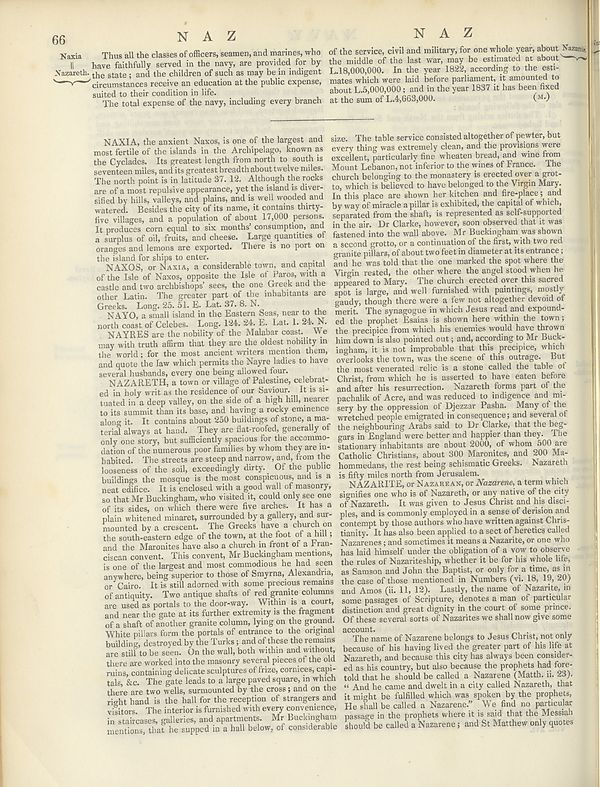
\includegraphics[width=0.85\textwidth]{../scans/page-1268-e5ec9e5b4086.jpg}
\caption*{Source scan: \texttt{page-1268-e5ec9e5b4086.jpg}}
\end{figure}

\end{document}
